\documentclass[10pt]{article}
\usepackage{geometry}
\usepackage{amsmath}
\usepackage{subfiles}
\usepackage{titleps}
\usepackage{multicol,caption}
\usepackage{enumerate}
\usepackage{listings}
\usepackage[toc,page]{appendix}
\usepackage{graphicx}
\usepackage{wrapfig}
\usepackage{algpseudocode}
\usepackage{algorithm}
\usepackage{xcolor}
\usepackage{pgfplots}
\usepackage{minitoc}
\usepackage[utf8]{inputenc}
\usepackage[english]{babel}
\usepackage{amsthm}
\pgfplotsset{compat=1.13}
\lstset{%
  title=\lstname,
  backgroundcolor=\color{white},
  basicstyle=\footnotesize,
  breakatwhitespace=false,
  breaklines=true,
  captionpos=b,
  commentstyle=\color{green},
  extendedchars=true,
  frame=single,
  keepspaces=true,
  keywordstyle=\color{blue},
  language=C++,
  numbers=left,
  numberstyle=\tiny\color{black},
  rulecolor=\color{black},
  showspaces=false,
  showstringspaces=false,
  showtabs=false,
  stepnumber=1,
  stringstyle=\color{magenta},
  tabsize=2
  }


\title{2D Graphics Rasterisation}
\author{Arden Rasmussen}

\begin{document}
\pagenumbering{gobble}
\maketitle
\pagenumbering{roman}
\begin{abstract}
   2D rasterisation is the process of converting rendering primitives such as
   polygons and lines, into a matrix of pixels or dots for output on a video
   display. This paper will look at the methods for rasterising several
   rendering primitives, such as lines, circles, and arbitrary polygons. This
   paper will also examine the methods for filling in the raster images
   generated from the rendering primitives.
\end{abstract}
\pagenumbering{arabic}
\section{Introduction}\label{sec:introduction}
   2D rasterisation is used to convert graphics primitives such as polygons and
   lines into a raster image. The raster image is a matrix of pixel, dot, or
   point data. These raster images can be used to output to a video display, or
   printer, or bitmap file formats. The rasterisation methods are necessary for
   determining what individual pixels of a display format must be set to.
   Because of this, rasterisation algorithms are found in all sorts of uses in
   computer science. This paper will examine some of the algorithms that are
   used for rasterisation of:
   \begin{enumerate}
     \item Lines
     \item Circles
     \item Polygons
   \end{enumerate}
   Along with a selection of algorithms that are used for filling polygons.

\section{Lines}\label{sec:lines}
  These algorithms are used to approximate a line segment on discrete graphical
  media. On the discrete graphical media, a line must be drawn as an
  approximation of the actual mathematical line segment in nontrivial cases.
  \subsection{Naive Line-Drawing}\label{sub:naive_line_drawing}
  \begin{algorithm}[H]
    \caption{Naive Line-Drawing}
    \begin{algorithmic}
      \State{\(d_x = x_2-x_1\)}
      \State{\(d_y = y_2-y_1\)}
      \For{$x \gets x_1$ to $x_2$}
      \State{$y = y_1+\frac{d_y\left(x-x_1\right)}{d_x}$}
      \State{\Call{Plot}{$x$,$y$}}
      \EndFor{}
    \end{algorithmic}
  \end{algorithm}
  This is only a valid algorithm if the points are already ordered such that
  $x_2 > x_1$. And it only works when $d_x \geq d_y$. To demonstrate the issues
  that are caused by this algorithm, here are several images depicting results
  of the algorithm.

\begin{minipage}{0.5\textwidth}
\begin{figure}[H]
  \centering
  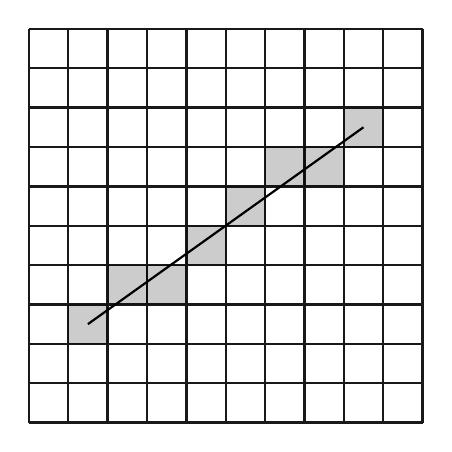
\begin{tikzpicture}[scale=0.5]
    \draw[step=1cm, line width=0.3mm, black!90!white] (0,0) grid (10cm,10cm);
    \draw[black,thick] (1.5,2.5)--(8.5,7.5);
    \filldraw[black,opacity=0.2](1,2)rectangle(2,3);
    \filldraw[black,opacity=0.2](2,3)rectangle(3,4);
    \filldraw[black,opacity=0.2](3,3)rectangle(4,4);
    \filldraw[black,opacity=0.2](4,4)rectangle(5,5);
    \filldraw[black,opacity=0.2](5,5)rectangle(6,6);
    \filldraw[black,opacity=0.2](6,6)rectangle(7,7);
    \filldraw[black,opacity=0.2](7,6)rectangle(8,7);
    \filldraw[black,opacity=0.2](8,7)rectangle(9,8);
  \end{tikzpicture}
  \caption{$d_x \geq d_y$}\label{fig:ld:nld:1}
\end{figure}
\end{minipage}\hfill
\begin{minipage}{0.45\textwidth}
  It can be seen that this algorithm can work effectivly for most cases where
  the slope of the line segment is less than or equal to $1$.
\end{minipage}

\begin{minipage}{0.5\textwidth}
\begin{figure}[H]
  \centering
  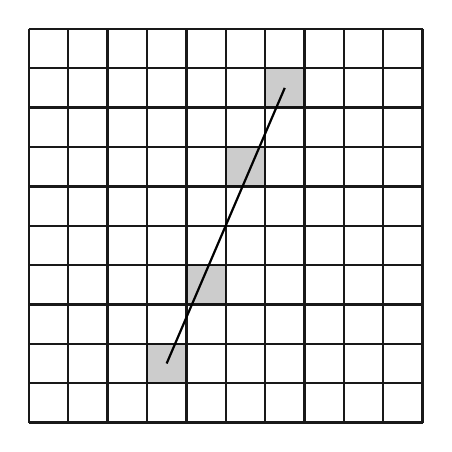
\begin{tikzpicture}[scale=0.5]
    \draw[step=1cm, line width=0.3mm, black!90!white] (0,0) grid (10cm,10cm);
    \draw[black,thick] (3.5,1.5)--(6.5,8.5);
    \filldraw[black,opacity=0.2](3,1)rectangle(4,2);
    \filldraw[black,opacity=0.2](4,3)rectangle(5,4);
    \filldraw[black,opacity=0.2](5,6)rectangle(6,7);
    \filldraw[black,opacity=0.2](6,8)rectangle(7,9);
  \end{tikzpicture}
  \caption{$d_x<d_y$}\label{fig:ld:nld:1}
\end{figure}
\end{minipage}\hfill
\begin{minipage}{0.45\textwidth}
  It can quickly be seen that when the slope of a line exceeds $1$, this algorithm quickly fails to draw compleate lines. And leaves large gaps between the pixels that it does draw.
\end{minipage}

Becaus of these reasons, this algorithm is rarly every used, and the other algorithms demonstrated are prefered.
\subsection{Digital Differential Analyzer (DDA)}\label{sub:digital_differential_analyzer}


\end{document}
